This section describes the purpose, use, and intended user audience for the Traffic Pi. Traffic Pi is a system that performs traffic study on its target area. A traffic study being described as analyzing the speed of vehicles entering its viewing area and recording this information in a centralized database. Users of Traffic Pi will be able to perform perform traffic studies by themselves using the product.

\subsection{Purpose and Use}
Traffic Pi will be able to analyze the speed of individual vehicles entering its view area and record this information to a centralized database. The expected use of Traffic Pi is for its user to direct the camera at the area of intent, turn on the device, and begin the traffic study on the targeted area.

\subsection{Intended Audience}
Traffic Pi is intended for individual citizens, groups, and/or entities that desire a traffic study of their local streets. The purpose of the traffic study is to learn more about the traffic patterns of their area, persuade the city to take action in mitigating risky behaviours by certain drivers, and/or effect safer driving habits by the city and public. While the intended audience for Traffic Pi is any individual or entity wanting to perform a traffic study by themselves, Traffic Pi has a narrow area of use as defined above.

\begin{figure}[h!]
	\centering
   	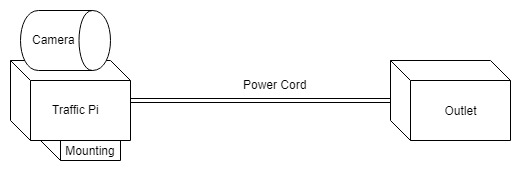
\includegraphics[width=0.90\textwidth]{images/Conceptual_Drawing.jpg}
    \caption{Traffic Pi conceptual drawing}
\end{figure}
